\chapter{Part 1}
\label{chap:Part1}
\section{Problem description}
As described above, the MovieLens dataset contains a lot of individual user ratings, but any good movie-site should present an average rating for each movie. Therefore, we will warm up by considering different ways of calculating average movie ratings.

Next, we consider a problem about pairing up movie-buddies. Based on the user�s individual ratings of movies, we wish to to pair up users, who for the most part have similar opinions on the movies which they have both rated. We will consider an approximation algorithm using MapReduce with the assumption that a large amount of data is to be processed.
\section{Average rating}
\subsection{Problem description}
The computation of average user ratings is in all its simplicity not a difficult algorithmic problem, but can, however, be addressed in several different ways. In the following we will discuss a na�ve sequential approach, a streaming approach and a MapReduce approach and end up with a comparison and an assessment.

\subsection{Problem description}
The computation of average user ratings is in all its simplicity not a difficult algorithmic problem, but can, however, be addressed in several different ways. In the following we will discuss a na�ve sequential approach, a streaming approach and a MapReduce approach and end up with a comparison and an assessment.

\subsection{Sequential approach}
The sequential approach is straightforward and will serve as a base case. The basic idea is to sum up all the ratings for each movie and divide by the number of ratings.

\[average = sum\_1\_to\_n( r1, ..., rn ) / n\]

This can be done in \(O(n)\) time and \(O(n)\) space. 
\subsection{Streaming approach}
If the amount of data is huge and user ratings keep coming in, the sequential algorithm might not be a viable approach. Instead, one could consider a simple streaming algorithm for computing the average movie ratings. 

\[stream: [ (movie\_id,rating)_0, (movie\_id,rating)_1, ..., (movie\_id,rating)_n\]

We imagine the user ratings arriving in a constant stream consisting of pairs of movie id�s and rating scores (the specific user who has rated the movie is not important in this example). The streaming algorithm then maintains a bin for each movie, containing the sum of the ratings seen so far, along with the total number of ratings processed concerning that specific movie. At anytime, an average movie rating can be retrieved by dividing the sum of ratings with the number of observations.

This approach requires \(O(m)\) space, where m is the total number of movies processed as there is a bin for each movie. The total amount of work is still \(O(n)\), and the time to retrieve an average rating is \(O(1)\), as it is a simple division of the two stored constants. 

Note that this is a naive streaming algorithm. Normally when using a streaming approach you would want a space requirement sublinear in the input size, however, if we want exact average ratings for each movie, we cannot do better than \(O(m)\) space.

\subsection{MapReduce approach}
In this case, we assume that a huge amount of data has already been collected, and therefore neither the sequential nor the streaming approach described above are viable. Also, we are operating a modern business, so of course we should exploit a cloud based solution. 

The approach we will use is MapReduce which is designed to work on distributed memory systems such as a cluster. The algorithm has a map step and a reduce step which together make up one round. Since the computation can be carried out in parallel on the cluster, the goal is to reduce the number of rounds and then, secondly, the total work. The algorithm we will use to compute the average movie ratings has a simple mapper and reducer and can be executed in a single round. 

The map function processes the input and emits pairs of movie id and rating. In between the map and reduce step, the pairs are shuffled, sorted by movie id and passed to the reducers. A reducer sums ratings and divide with the number of ratings for that particular movie. There can be an arbitrary number of mappers and a maximum of m reducers, where m is the total number of movies.

\begin{center}
\begin{tabular}{ r  l  }
Total work:& \(O(n)\)\\
Total work per reducer:& \(O(\)maximum number of ratings for one movie\()\)\\
Amount of pairs:&                \(O(n)\)\\ 
Number of rounds:&               \(O(1)\)\\ 
\end{tabular}
\end{center}

\subsection{Implementation}
We have implemented all three approaches of computing the average ratings in Java for demonstration. The sequential and streaming approaches are rather straight forward. Applying the MapReduce approach was a bit of a struggle as it took some time setting up Hadoop,, but the algorithm itself is pretty simple. The code can be found on the enclosed CD.

\section{Movie buddies}
\subsection{Problem description}
As mentioned in the introduction to this part, we want to find a way to pair up users based on their individual movie ratings, i.e. we want to find a maximum matching, minimizing the rating difference on movies rated by each pair of users. We call such a pair movie buddies. 

The graph we constructed for this problem has users as vertices. A pair of vertices are connected with an undirected edge if the two users have rated one or more of the same movies. Additionally, each edge will be assigned a weight defined as the total difference in the score of the ratings divided by the number of movies that have been rated by both users. We will use this weight as a measure of how similar the movie taste of the two users is

\[weight = sum\_1\_to\_n(5 - | r^i_1 - r^i_2 | ) / n\]

where \(n\) is the number of movies rated by both users, and \(r_i^1\) and \(r_i^2\) are the individual ratings given by the two users on the same movie, denoted with the number i. 

This is can be categorized as a maximum weighted matching problem. A matching is defined as a set of edges without common vertices. A \emph{maximum matching} is a matching containing the largest possible number of edges and a \emph{maximal matching} is a matching M with the property that if any edge is added to M it is no longer a valid matching. In a \emph{maximum weighted matching}, we want to maximize the sum of the weights of the matched edges.

In the following we describe two different approaches to solving this problem. First a sequential approach and then we discuss how the problem may be solved in a parallel, distributed way, assuming the graph is very large.

\subsection{Sequential algorithm}
The applied sequential algorithm is a linear time \(\frac{1}{2}\)-approximation algorithm (LAM) for maximum weighted matching used in general graphs \cite{robert}.

\subsubsection{Motivation}
The goal of using this algorithm is to find a maximum weighted matching (MWM). The optimal solution to this algorithmic problem is a polynomial time algorithm which was first designed by J. Edmonds in 1965\cite{edmonds} using polynomial time. LAM gives an approximated solution in a linear computation time. It will provide a great advantage in the running time of larger datasets as the one we are using.

\subsubsection{Description of the algorithm}
The following pseudo-code outlines the structure of the algorithm.

\begin{lstlisting}
LAM-Algorithm
MLAM := �;
WHILE (E�)
    take the locally heaviest edge {a,b}E;
    add {a,b} to MLAM;
remove all edges incident to a or b from E;
ENDWHILE
\end{lstlisting}

The algorithm starts with an empty matching \(M_{LAM}\) in which the edges recursively will be added during the execution and a set \(E\) containing all the edges between the vertices in the graph. It initiates by choosing an arbitrary edge \(e=\{a,b\}\) from E and starts checking if any of the adjacent edges to the two vertices a and b have a higher weight than e. If such an edge is found it proceeds to that edge and applies the procedure. It continues until an edge is found where no adjacent edges have a higher weight than the current one. When the edge with the locally highest weight is found, it is added to \(M_{LAM}\) and all edges incident to the two vertices of the edge are removed from \(E\). The algorithm terminates when \(E\) is empty.

Figure \ref{fig:edge_figure} gives an example of the process of the algorithm. The algorithm has traversed through edge 1 and 2 and is currently at edge 3. It applies that \(edge 1 < edge 2 < edge 3.\) It checks if the edges incident to a and b are of higher weight than {a,b} and adds it to \(M_{LAM}\). Thus, the edges \({a,c_{1,2,3}} < {a,b}\) and \({b, d_{1,2}} < {a,b}\).

\begin{figure}[h]
  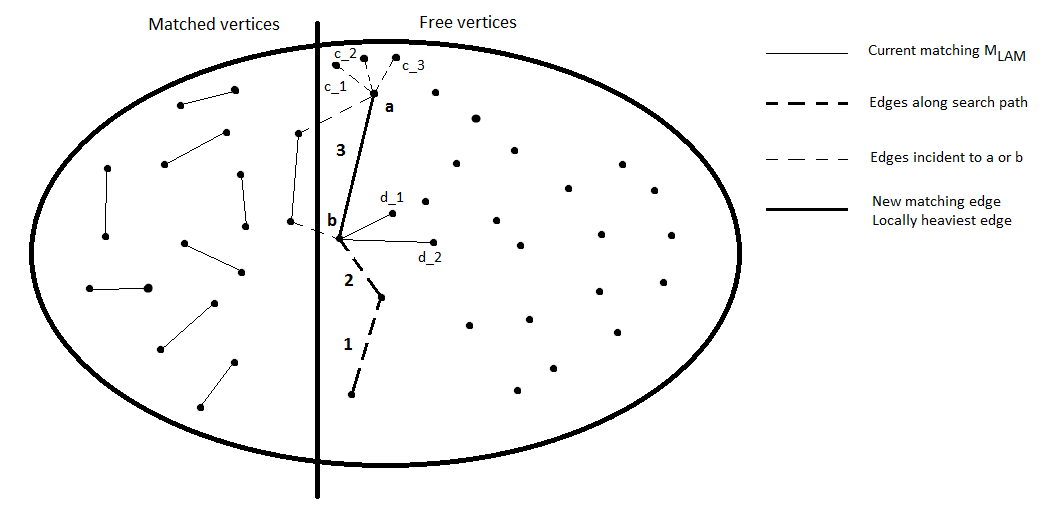
\includegraphics[width=300pt]{edge_figure.png}
\caption{An example of the LAM process. The figure is from \cite{robert}}
\label{fig:edge_figure}
\end{figure}

\subsection{Running time}
The running time of the algorithm is linear and thus it is ideal to use on large datasets. Proofing the running time of the algorithm is quite simple as every iteration of the while loop removes at least one edge and thus the total amount of iterations and removed edges cannot exceed \(O(|E|)\).

\subsection{Advantages and disadvantages}
This algorithm does not find an optimal MWM, but guarantees to find a matching that contains at least half the weight of an optimal solution. The formal proof of the approximation can be found in chapter 3 in \cite{robert}.

It is not possible to apply parallel computation on the algorithm as the process of the algorithm is based on two recursive calls (on a and b) which then would not know if the other recursive call had already processed a given edge. It would result in a collision between the edges matched in the recursive calls.

This algorithm does not give the best running time for the algorithmic problem it solves, but it is a rather simple algorithm to understand and apply. Later during the project we found better algorithms to solve the MWM problem. This was for instance the near-linear time \((1-\epsilon)\) -approximation algorithm for MWM\cite{duan} which provides a solution closer to optimal.

\subsection{Distributed algorithm}
The graph we are considering may potentially be too large to be kept in memory and processed by a sequential algorithm. Here we consider a MapReduce approach exploiting a technique called filtering \cite{filtering}. The main idea behind filtering is to reduce the size of the input in a distributed manner, so that the resulting considerably smaller input can be solved on a single machine. This approach works specifically for sufficiently dense graphs where the number of edges is much larger than the number of vertices. 

We will start out by presenting an algorithm to compute an unweighted maximal matching and thus a 2-approximation to the unweighted maximum matching problem. Then we will extend this technique to obtain an 8-approximation algorithm to the maximum weighted matching problem\cite{filtering}. Please note that some details have been left out for the sake of simplicity.

Let \(G=(V,E)\) be an undirected graph, where \(n=|V|\) and \(m=|E|\). We will call G c-dense if \(m=n^{1+c}\), where \(0<c<=1\). We assume the machines we are working with have a limited memory of size s. 

\subsubsection{Unweighted maximal matching}
First we consider an algorithm for solving an unweighted maximal matching problem on a large graph, G. The algorithm operates by first sampling \(O(s)\) edges from G and finding a maximal matching M� in the resulting subgraph and then augmenting the final matching M with M�. Given M, we can now safely remove edges from G that are in conflict with M. If the resulting filtered graph, G�, can fit in memory on a single machine, the algorithm augments M with a matching found on G� and returns the final matching, M. Otherwise, we augment M by recursing on G�. Please refer to \cite{filtering} for the formal description of the algorithm.

We claim that the algorithm returns a maximal matching. For the sake of contradiction, consider an edge (u,v) in E such that neither u nor v are matched in M. In the last iteration of the algorithm, a maximal matching, M�, is found on the set of edges that are not in conflict with M, and M is augmented with M�. Since M� is a maximal matching, either u, v or both must be in M� and therefore in the final matching M. This gives us our contradiction and therefore the final matching M is a maximal matching on G.

Now we show that the algorithm can be implemented in three MapReduce rounds with high probability when \(s=n^{1+2c/3}\) and at most O(log n) rounds. In \cite{filtering} it is shown that the algorithm runs for one iteration with high probability when \(s=n^{1+2c/3}\) and O(log n) rounds otherwise. Therefore it only remains to describe how to compute G�, the filtered subgraph with the edges not in conflict with the initial matching. Denote by \(S_i\), a subset of E, the edges incident on node i, and let \(f_i\) be a function that drops an edge if it is matched and keeps it otherwise. The collection of functions \(f_i\) can be parallelized and computed in one MapReduce round. This is drawn from Lemma 6.1 in \cite{model}, which presents a model for computation in MapReduce. 

\subsection{Maximum weighted matching}
We now consider the algorithm for computing an 8-approximation of the weighted maximum matching problem \cite{filtering}. The input to this algorithm is a simple graph, G=(V,E), and a weight function \(w : E \to R\). Denote by W the maximum weight.

The Algorithm operates as follows: Split G into \(G1,G2, ...  ,G_{ceil(log W)}\), where Gi is the graph on the set V of vertices and the subset of edges in E with weights from \(2^{i-1}\) to \(2^{i}\). For \(1 \leq i \leq ceil(log W)\) run the maximal matching algorithm described above on \(G_i\) and let \(M_i\) be the matching for \(G_i\). Now consider the matchings in descending order from M\(_{ceil(log W)}\) to \(M_1\). When considering an edge e in \(M_i\), we add it to the final matching M if \(M \cup {e}\) is a valid matching, i.e if e is not in conflict with any other edge already in M. After all edges are considered, return M.

The above algorithm is an 8-approximation to the weighted maximum matching problem. Let OPT be the optimal solution on G. Let e=(u,v) belong to OPT and e belong to \(G_j\) for some j. Since we are selecting edges from the matchings in descending order, we might pick an edge from \(M_i\) for \(i \geq j\) incident on either u or v such that e is blocked and cannot be picked later. It can be shown that:

\[ \sum_{(u,v)\in M} w((u,v)) \geq \sum_{e\in OPT} w(e) \]
We refer to Lemma 3.4 in \cite{filtering} for the full proof.

Note that it is possible to run the above algorithm in MapReduce using only one more round than the maximal matching algorithm. In the first round we split up G into \(G1,G2, ...  ,G_{ceil(log W)}\), then we run the maximal matching algorithm in parallel on \(ceil(log W)\) machines. In the last round, we run the last step on a single machine resulting in a final matching M. 


